\subsection*{Task 4}

\subsubsection*{b)}

\begin{figure}[h!]
  \centering
  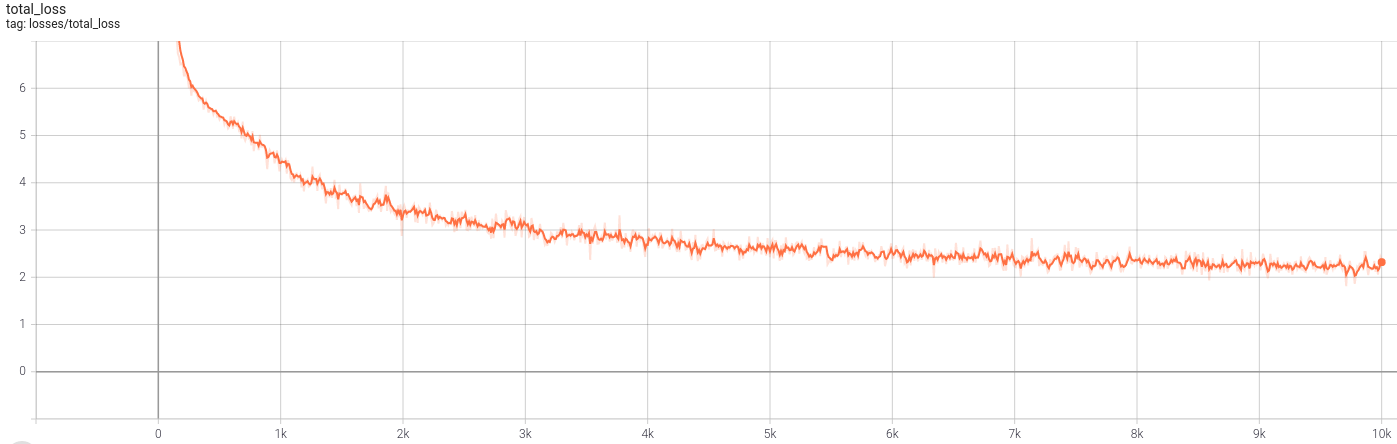
\includegraphics[width=\textwidth]{figures/total_loss.png}
  \caption{Total loss over 10k iterations.}
  \label{fig:task4:b}
\end{figure}

After 10k gradient descent iterations the mean average precision was 0.8004.


\subsubsection*{c) and d)}

The improved model is found in \texttt{ssd/modeling/backbone/improved.py} with config \texttt{mnist\_improved.yaml}. 

From Assignment 3 I saw that batch normalization contributed greatly to the overall performance, which was therefore added after each convolutional layer. I also switched to the Adam optimizer, and set the learning rate to $5\cdot10^{-4}$. One more convolutional layer (with batch normalization and ReLU) was also added to each feature map. This gave a mAP of around 85\% within 10k iterations. After running \texttt{demo.py} I saw that the network struggled with smaller scales, so I added a $76\times76$ feature map for detecting numbers with smaller scale. This finally gave a mAP of 0.9047 after 14k iterations, barely achieving the goal. Output from \texttt{test.py} with the network is shown in \cref{fig:task4:d}. The mAP over all iterations is shown in \cref{fig:task4:d_map}, where we see that the actual mAP barely reaches 90\% at iteration 14k. The total loss is shown in \cref{fig:task4:d_loss}.

\begin{figure}[h!]
  \centering
  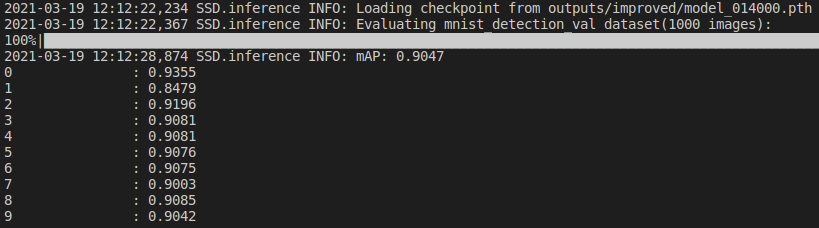
\includegraphics[width=\textwidth]{figures/Task4c.png}
  \caption{Output of \texttt{test.py} at checkpoint from iteration 14k.}
  \label{fig:task4:d}
\end{figure}

\begin{figure}[h!]
  \centering
  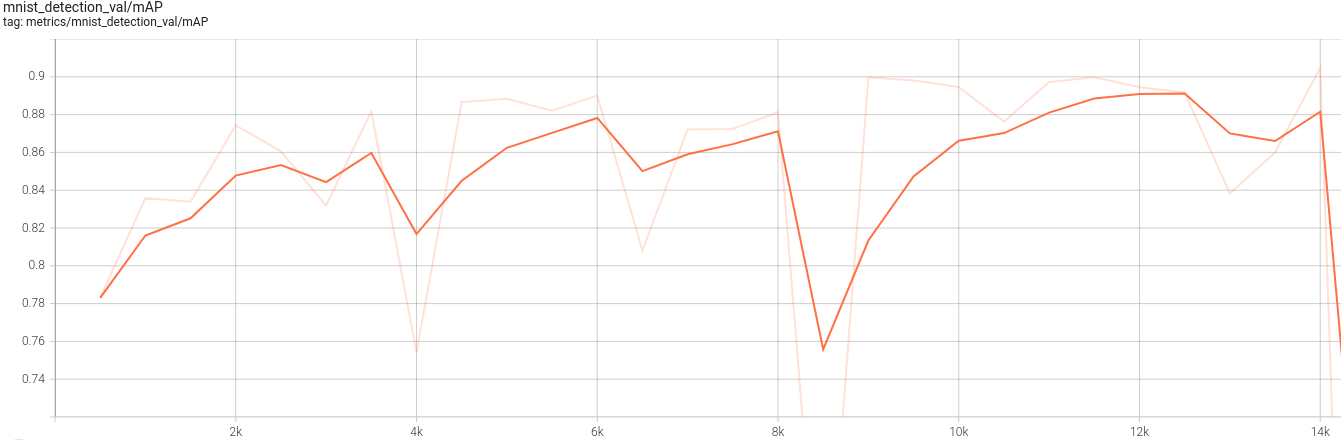
\includegraphics[width=\textwidth]{figures/Task4e_mAP.png}
  \caption{mAP over all iterations, with smoothed value as strong line and actual value as weak line.}
  \label{fig:task4:d_map}
\end{figure}

\begin{figure}[h!]
  \centering
  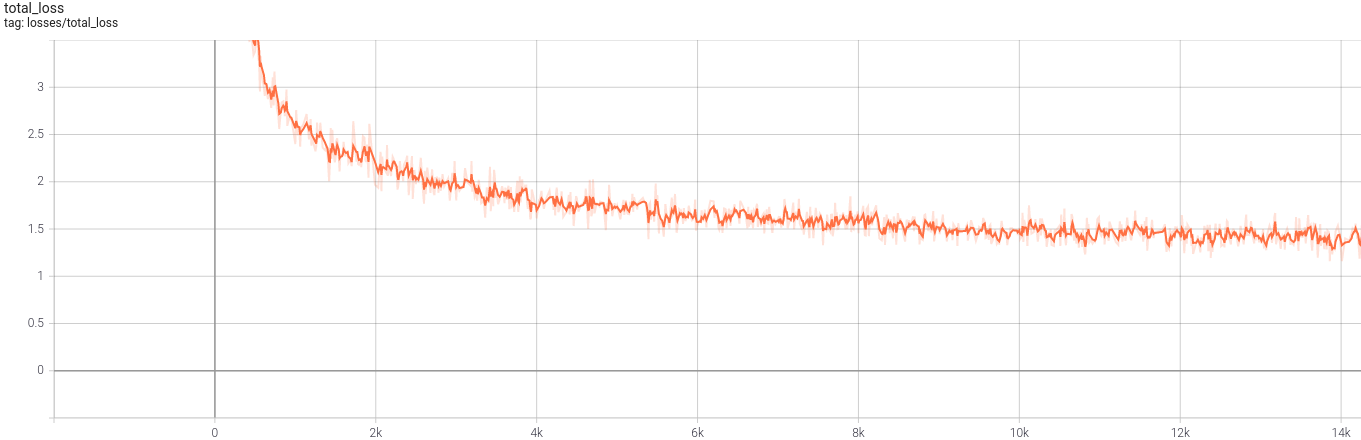
\includegraphics[width=\textwidth]{figures/Task4d_loss.png}
  \caption{Total loss over all iterations..}
  \label{fig:task4:d_loss}
\end{figure}

\newpage
\subsubsection*{e)}

The results from \texttt{demo.py} with the model from d) is shown in \cref{fig:task4:e1}, \cref{fig:task4:e2} and \cref{fig:task4:e3}. We see that the model struggles with numbers that have smaller scale, and mostly with the digit "1" or numbers that resemble "1". The $76\times76$ feature map did thus not solve the problem completely, and in afterthought a better solution may be to modify the bounding box parameters instead, to give smaller default bounding boxes. 

\begin{figure}
  \centering
  \begin{subfigure}[b]{0.49\textwidth}
    \centering
    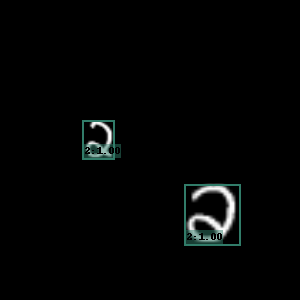
\includegraphics[width=\textwidth]{figures/0.png}
  \end{subfigure}
  \begin{subfigure}[b]{0.49\textwidth}
    \centering
    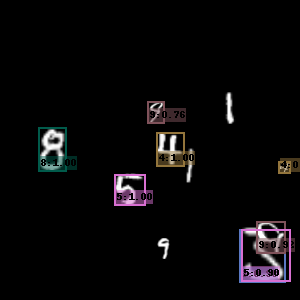
\includegraphics[width=\textwidth]{figures/1.png}
  \end{subfigure}
  ~
  \begin{subfigure}[b]{0.49\textwidth}
    \centering
    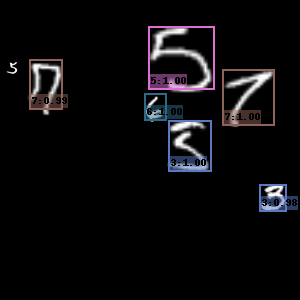
\includegraphics[width=\textwidth]{figures/2.png}
  \end{subfigure}
  \begin{subfigure}[b]{0.49\textwidth}
    \centering
    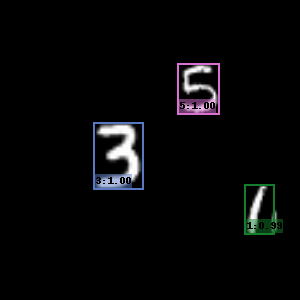
\includegraphics[width=\textwidth]{figures/3.png}
  \end{subfigure}
  ~
  \begin{subfigure}[b]{0.49\textwidth}
    \centering
    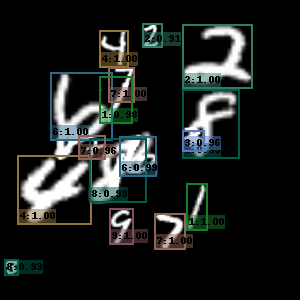
\includegraphics[width=\textwidth]{figures/4.png}
  \end{subfigure}
  \begin{subfigure}[b]{0.49\textwidth}
    \centering
    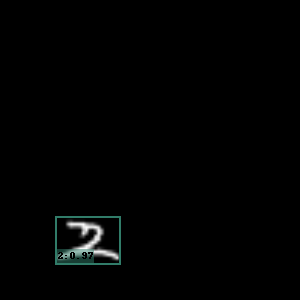
\includegraphics[width=\textwidth]{figures/5.png}
  \end{subfigure}
  \caption{Images 0-5.}
  \label{fig:task4:e1}
\end{figure}

\begin{figure}
  \centering
  \begin{subfigure}[b]{0.49\textwidth}
    \centering
    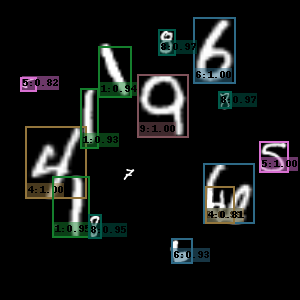
\includegraphics[width=\textwidth]{figures/6.png}
  \end{subfigure}
  \begin{subfigure}[b]{0.49\textwidth}
    \centering
    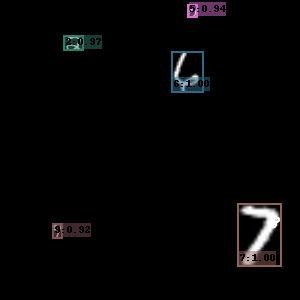
\includegraphics[width=\textwidth]{figures/7.png}
  \end{subfigure}
  ~
  \begin{subfigure}[b]{0.49\textwidth}
    \centering
    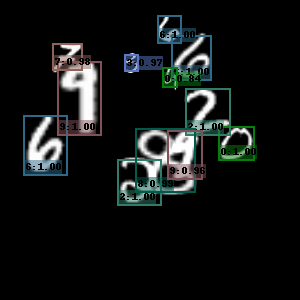
\includegraphics[width=\textwidth]{figures/8.png}
  \end{subfigure}
  \begin{subfigure}[b]{0.49\textwidth}
    \centering
    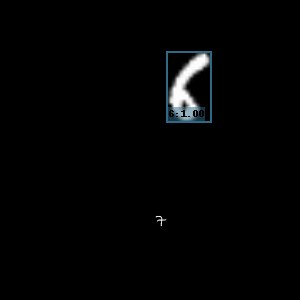
\includegraphics[width=\textwidth]{figures/9.png}
  \end{subfigure}
  ~
  \begin{subfigure}[b]{0.49\textwidth}
    \centering
    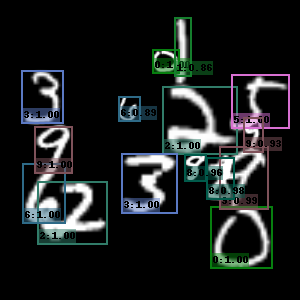
\includegraphics[width=\textwidth]{figures/10.png}
  \end{subfigure}
  \begin{subfigure}[b]{0.49\textwidth}
    \centering
    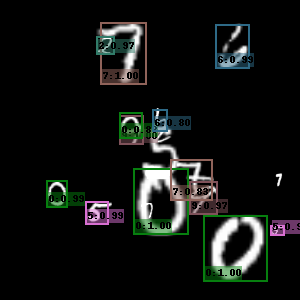
\includegraphics[width=\textwidth]{figures/11.png}
  \end{subfigure}
  \caption{Images 6-11.}
  \label{fig:task4:e2}
\end{figure}

\begin{figure}
  \centering
  \begin{subfigure}[b]{0.49\textwidth}
    \centering
    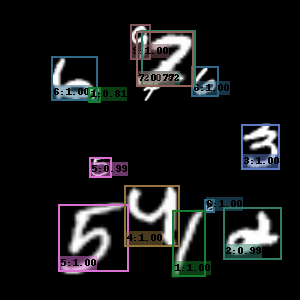
\includegraphics[width=\textwidth]{figures/12.png}
  \end{subfigure}
  \begin{subfigure}[b]{0.49\textwidth}
    \centering
    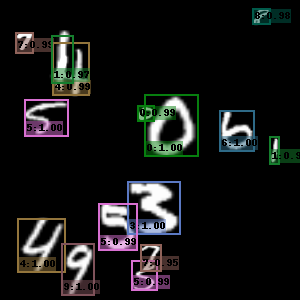
\includegraphics[width=\textwidth]{figures/13.png}
  \end{subfigure}
  ~
  \begin{subfigure}[b]{0.49\textwidth}
    \centering
    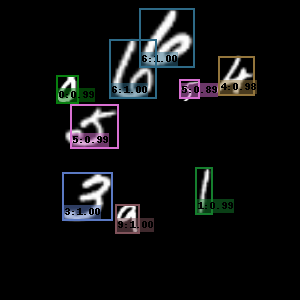
\includegraphics[width=\textwidth]{figures/14.png}
  \end{subfigure}
  \caption{Images 12-14.}
  \label{fig:task4:e3}
\end{figure}


\subsubsection*{f)}

Despite fixing the errors in the original config, I was not able to achieve a mAP higher than 0.2409, as seen from \cref{fig:task4:f_map}. The predictions did therefore not give any good results, and I had to lower the threshold for accepting a bounding box to 0.4 to show any results at all. Total loss is shown in \cref{fig:task4:f_loss}.

\begin{figure}[h!]
  \centering
  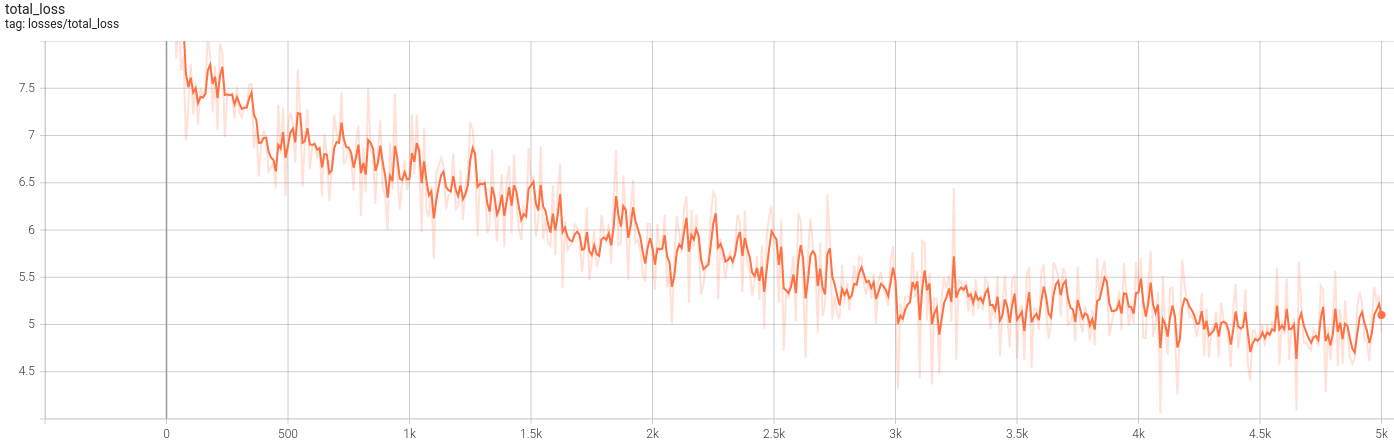
\includegraphics[width=\textwidth]{figures/Task4f_loss.png}
  \caption{Total loss.}
  \label{fig:task4:f_loss}
\end{figure}

\begin{figure}[h!]
  \centering
  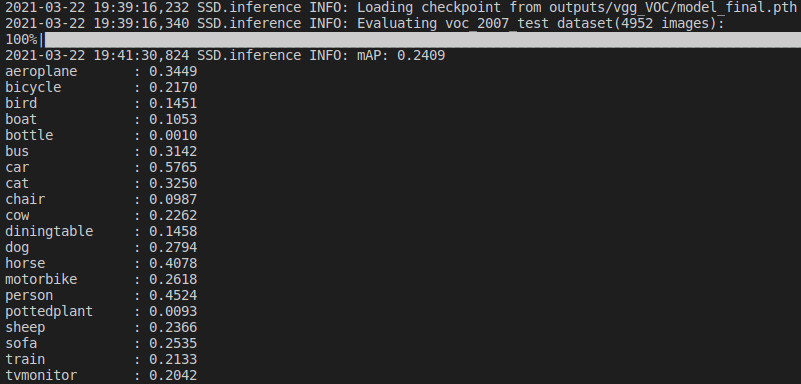
\includegraphics[width=\textwidth]{figures/Task4f_map.png}
  \caption{Output of \texttt{test.py}.}
  \label{fig:task4:f_map}
\end{figure}

\begin{figure}[h!]
  \centering
  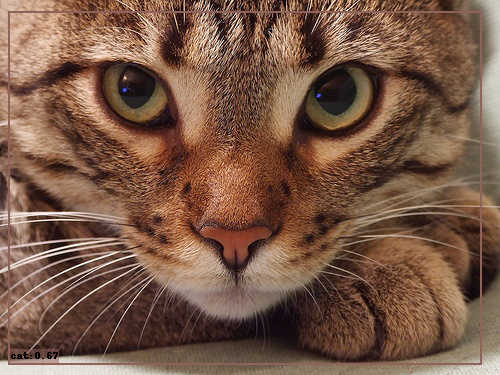
\includegraphics[width=0.5\textwidth]{figures/000542.png}
\end{figure}

\begin{figure}[h!]
  \centering
  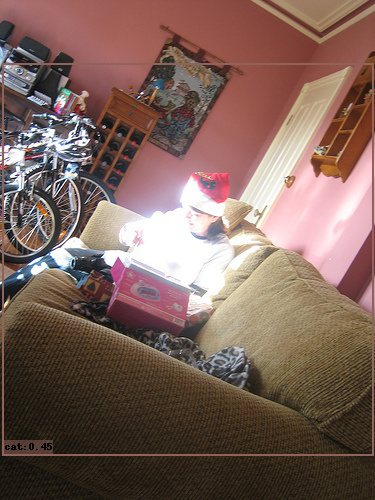
\includegraphics[width=0.5\textwidth]{figures/004101.png}
\end{figure}

\begin{figure}[h!]
  \centering
  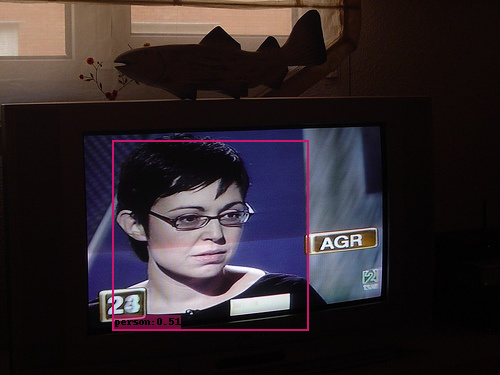
\includegraphics[width=0.5\textwidth]{figures/000342.png}
\end{figure}

\begin{figure}[h!]
  \centering
  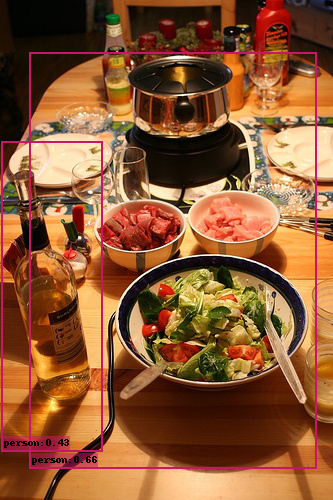
\includegraphics[width=0.5\textwidth]{figures/008591.png}
\end{figure}

\begin{figure}[h!]
  \centering
  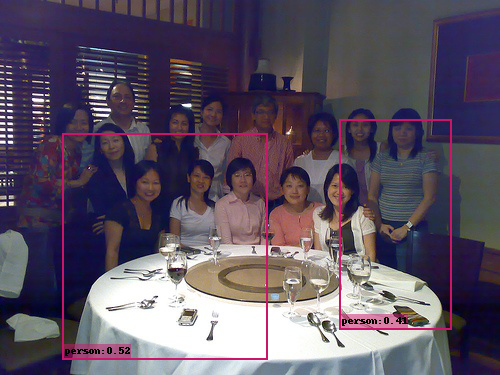
\includegraphics[width=0.5\textwidth]{figures/003123.png}
\end{figure}


